%!TEX root=../main.tex

\section{Introduction} % (fold)
\label{sec:introduction}

We extend our congratulations to \cite{happMultivariateFunctionalPrincipal2018} for their outstanding article. Despite the substantial interest on dimension reduction in the (multivariate) functional data literature, we concur with the authors that existing methods are often limited to either univariate functional data or multivariate functional data defined on a common one-dimensional domain. However, research has introduced a growing presence of data defined on different dimensional domains, such as curves and surfaces, observed in diverse fields, including neuroscience, biomechanics, and other domains. In this discussion, we aim to provide commentary on the estimation of the number of principal components utilising the methodology devised by the authors. To achieve this, we conducted an extensive simulation study and subsequently propose practical guidelines for practitioners to adeptly chose the appropriate number of components for multivariate functional datasets. For ease of presentation, we use the same notation as theirs. Code to reproduce the simulation study in this discussion is available at \url{https://github.com/FAST-ULxNUIG/variance_mfpca}.

% section introduction (end)

\section{Model} % (fold)
\label{sec:model}

\cite{happMultivariateFunctionalPrincipal2018} proposed an extension of functional principal components analysis (\cite{ramsayFunctionalDataAnalysis2005}) to multivariate functional data, named multivariate functional principal components analysis (MFPCA). 

\textcolor{red}{We briefly present the estimation of MFPCA. For a detailled description of the estimation process, see \cite[Section 3]{happMultivariateFunctionalPrincipal2018}. In \cite{happMultivariateFunctionalPrincipal2018}, the authors first estimate the principal components for each individual feature and combine them to derive the multivariate components. So, they chose a number of components for each individual feature and then use only these ones to compute the multivariate components. Let $K_p$ be the number of components retained for the $p$th feature. As the univariate components are concatenated to estimated the multivariate components, the number of multivariate components that can be estimated is $\sum_p K_p$. We however claim that only $\min_p K_p$ can only be accurately estimated.
The estimation of the number of components can also be done using the percentage of variance explained. 
We are interested by the estimation of the eigenvalues of functional datasets. Let $\{\nu_k\}_{1 \leq k \leq K}$ be the set of true eigenvalues and $\{\widehat{\nu}_k\}_{1 \leq k \leq K}$ be the set of estimated eigenfunctions. Simulations are the same as the first setting in \cite{happMultivariateFunctionalPrincipal2018}. The accuracy of the resulting estimates $\widehat{\nu}_j$ is measured by the relative errors $\text{Err}(\widehat{\nu}_j)  = (\nu_j - \widehat{\nu}_j)^2 / \nu^2_j$. The percentage of variance explained by the $k$th component is defined as
\begin{equation}\label{eq:pve}
     \text{PVE}_k = \frac{\nu_k}{\sum_{k = 1}^K \nu_k}.
\end{equation}
The cumulative percentage of variance explained by the first $k$ components is given by
\begin{equation}\label{eq:cum_pve}
     \text{PVE}_{1:k} = \frac{\sum_{l = 1}^k \nu_l}{\sum_{l^\prime = 1}^K \nu_{l^\prime}}.
\end{equation}
Given a certain percentage of variance explained $\alpha$, the number of components needed to explain at least $\alpha\%$ of the variance of the data is
\begin{equation}\label{eq:npc}
     \text{NPC}_{\alpha} = \sum_{k = 1}^K \mathbf{1}\left\{\text{PVE}_{1:k} < \alpha\right\} + 1 = \min_{k = 1, \dots, K} \text{PVE}_{1:k} > \alpha.
\end{equation}}

% section model (end)

\section{Simulation} % (fold)
\label{sec:simulation}

We perform a simulation study based on the first setting in the simulation in \cite{happMultivariateFunctionalPrincipal2018}. The data-generating process is based on a truncated version of the Karhunen-Loève decomposition. First, we generate a large orthonormal basis $\{\psi_m\}_{1 \leq k \leq M}$ of $\sLp{\TT{}}$ on an interval $\TT{} = [0, T] \subset \RR$. We fix $T_1 = 0$ and $T_{p + 1} = T$ and we generate $p - 1$ cutting points $T_2, \dots, T_p$ uniformly in $\TT{}$ such that $0 = T_1 < \cdots < T_p < T_{p+1} = T$. Let $s_1, \dots, s_p \in \{-1, 1\}$ be coefficients that randomly flip the eigenfunctions with probability $0.5$. The univariate components of the eigenfunctions are then defined as
\begin{equation}\label{eq:simulation_uni_component}
    \psi_m^{(j)}(t_j) = s_j \restr{\psi_m}{[T_j, T_{j + 1}]}\left(\frac{t_j - T_j}{T_{j + 1} - T_j}\right), \quad m = 1, \dots, M, \quad j = 1, \dots, p.
\end{equation}
The notation $\restr{\psi_m}{[T_j, T_{j + 1}]}$ is the restriction of the function $\psi_m$ to the set $[T_j, T_{j + 1}]$. The set of multivariate functions $\{\psi_m\}_{1 \leq m \leq M}$ is an orthonormal system in $\HH \coloneqq \sLp{\TT{1}} \times \dots \times \sLp{\TT{p}}$ with $\TT{j} = [0, 1]$. Each curve is then simulated using the truncated multivariate Karhunen-Loève expansion:
\begin{equation}
    x_i(\pointt) = \sum_{m = 1}^M \rho_{i, m} \psi_m(\pointt), \quad \pointt \in \TT{},\quad i = 1, \dots, N,
\end{equation}
where the scores $\rho_{i, m}$ are sampled as random normal variables with mean $0$ and variance $\nu_m$. The eigenvalues $\nu_m$ are defined with an exponential decrease, $\nu_m = \exp(-(m + 1)/2)$. We simulate, for each replication of the simulation, $N = 25, 50$ and $100$ observations. Similarly, each component is sampled on a regular grid of $S = 25, 50$ and $100$ sampling points. We use $p = 5$ features and we set $M = 50$. The estimation is done using the \textsf{R} package \texttt{MFPCA} \citep{happ-kurzObjectOrientedSoftwareFunctional2020}. For each univariate feature $j$, we estimate $M_j = 5$ principal components. Then, following the multivariate components estimation procedure, we can estimate $\sum_{j = 1}^p M_j = 25$ multivariate components. 

The outcomes concerning the errors in estimating the eigenvalues are displayed in Figure \ref{fig:ncomp}. Notably, the accuracy of the estimation diminishes with an increasing number of components in all scenarios. While there is a distinct jump in accuracy observed for the last five estimated eigenvalues, establishing a general rule proves challenging. It is worth emphasizing that the number of multivariate eigencomponents to be estimated is $\min_p K_p$; otherwise, the univariate components lack sufficient information to accurately recover their corresponding multivariate counterparts.
\begin{figure}
     \centering
    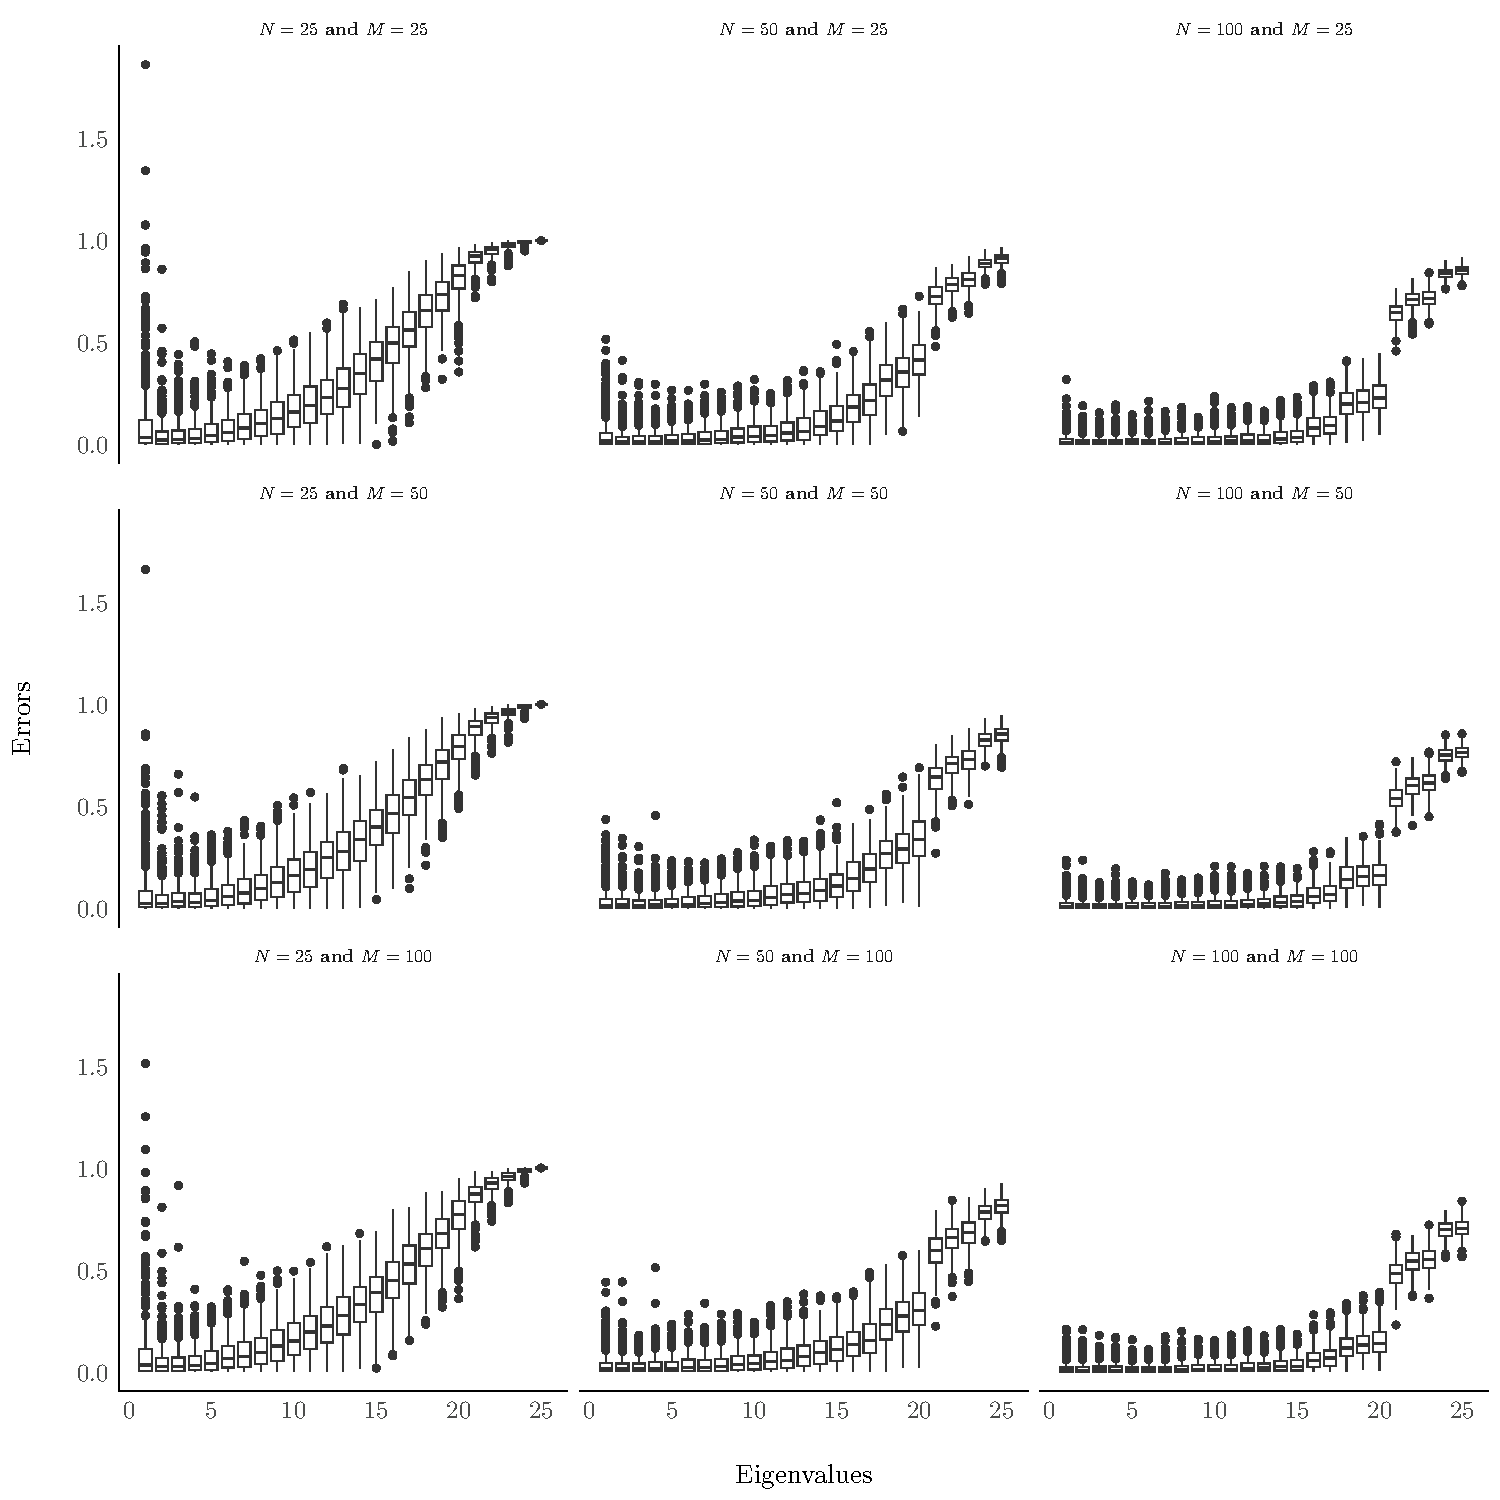
\includegraphics[width=0.95\textwidth]{figures/ncomp.pdf}
    \caption{Boxplots of the estimation errors of the eigenvalues. We estimated $5$ components for each univariate feature. The number of multivariate eigencomponents that can be estimated is thus $25$. $N$ is the number of observations, $S$ is the number of sampling points per curve. We run $500$ simulations.}
    \label{fig:ncomp}
\end{figure}
Figure \ref{fig:npc_estim} showcases the estimation of the number of components retained across $500$ simulation scenarios for a fixed percentage of variance explained. The red dots represent the number of components that should be retained for $\alpha\%$ of variance explained, considering an exponential decay of the eigenvalues as defined in equation \eqref{eq:npc}. Additionally, the size of the black dots indicates the frequency of selection for each component over the $500$ simulations. Notably, the number of components appears to be consistently underestimated for various combinations of the number of observations $N$, number of sampling points $S$, and desired percentage of variance explained $\alpha\%$. These findings may hold considerable significance for practitioners.
\begin{figure}
     \centering
    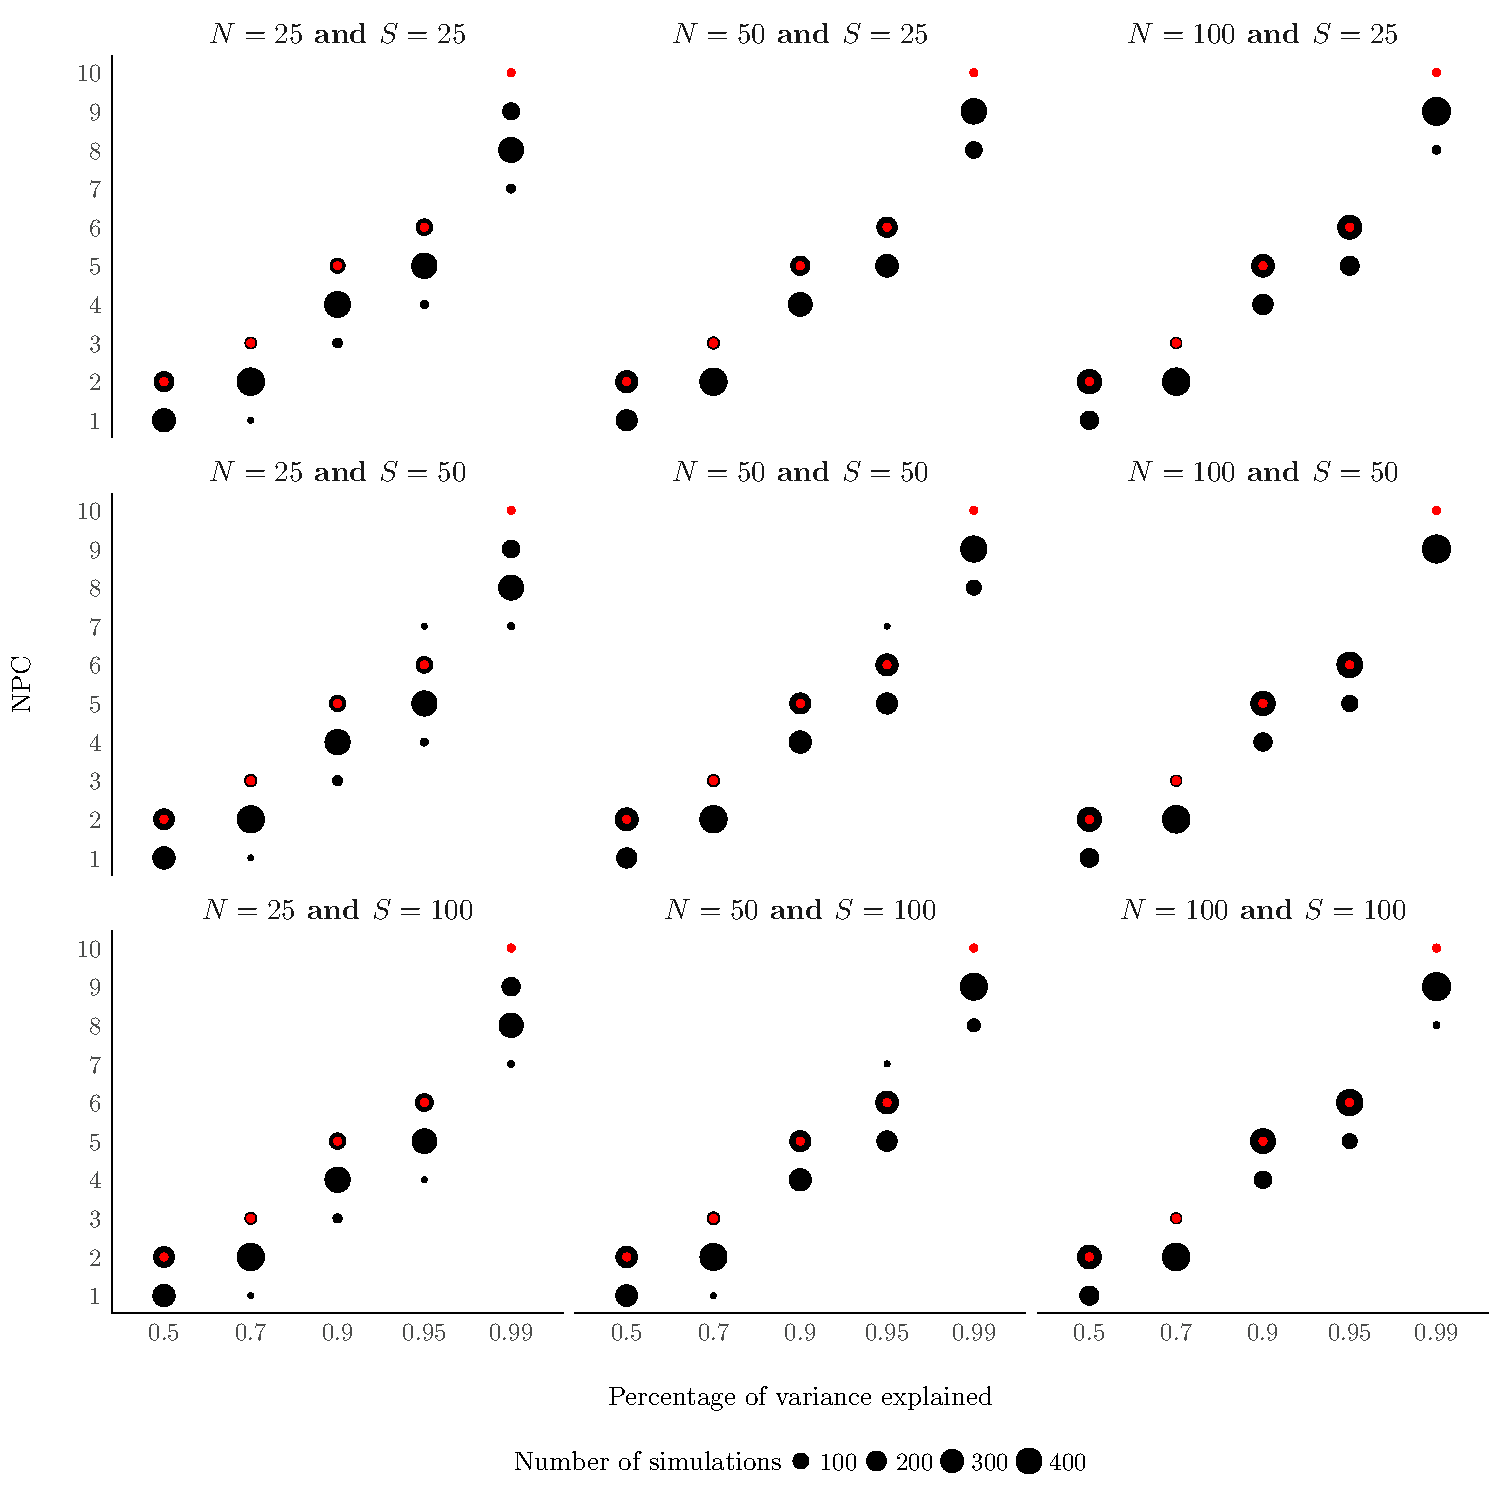
\includegraphics[width=0.95\textwidth]{figures/npc_estim.pdf}
    \caption{The size of the black dots represents the number of times the number of components has been selected over $500$ simulations. The red dots are the true number of components given the percentage of variance explained. $N$ is the number of observations, $S$ is the number of sampling points per curve.}
    \label{fig:npc_estim}
\end{figure}

% section simulation (end)

\section{Conclusion} % (fold)
\label{sec:conclusion}

\cite{happMultivariateFunctionalPrincipal2018} presents a general methodology to estimate principal components for a set of multivariate functional data defined on, possibly, different dimensional domains. Their approach, based on the decomposition of the covariance of each univariate feature, allows easy inference of the components.

We conducted a simulation study, and the obtained results highlight two important findings. Firstly, although utilizing only a few univariate components may yield a substantial number of multivariate components, their accuracy is notably limited. Secondly, relying on the percentage of variance explained as a criterion for selecting the number of components may result in an underestimation of this number. We, therefore, advise practitioners to exercise caution when determining the number of estimated components. It is prudent to refrain from utilizing more than $\min_j M_j$ estimated multivariate components. Additionally, we strongly recommend conducting simulations that closely resemble the characteristics of the actual data to select the appropriate number of components based on the percentage of variance explained criterion.

% section conclusion (end)





